\documentclass{csse4400}

\usepackage{tikz}
\usetikzlibrary{positioning}
\usetikzlibrary{arrows}

\usepackage{float}

\usepackage{enumitem}

\usepackage{languages}

\title{Pipeline Architectures}
\author{Brae Webb}

\date{\week{2}}
\begin{document}

\maketitle

\section{Brief}
This week we are looking into architectures which
follow the pipeline architectural style.
Specifically, this week we will:
\begin{enumerate}
    \item Briefly recap the concepts of pipeline architectures.
    \item Explore the advantages of using bash as a well-implemented pipeline architecture using the Knuth/McIlroy example.
    \item Explore whether compilers are a suitable pipeline architecture.
    \item Briefly look at one of the primary modern applications of the pipeline style,
        MapReduce.
\end{enumerate}

\section{Case Study: Compilers}

An interesting case study of the pipeline architecture is a compiler.%
\footnote{You do not need to understand the phases of a compiler --- two data structures, the Symbol Table and Abstract Syntax Tree (AST), are transformed in each compiler phase.}
As a foundational technology, compilers have undergone rigorous refinement and are perhaps the most well studied type of software.
Modern compilers have well-defined modular phases as illustrated by Figure \ref{fig:compiler-architecture},
each phase of a compiler transforms the representation of the program until the target program is produced.

\begin{figure}[H]
    \centering
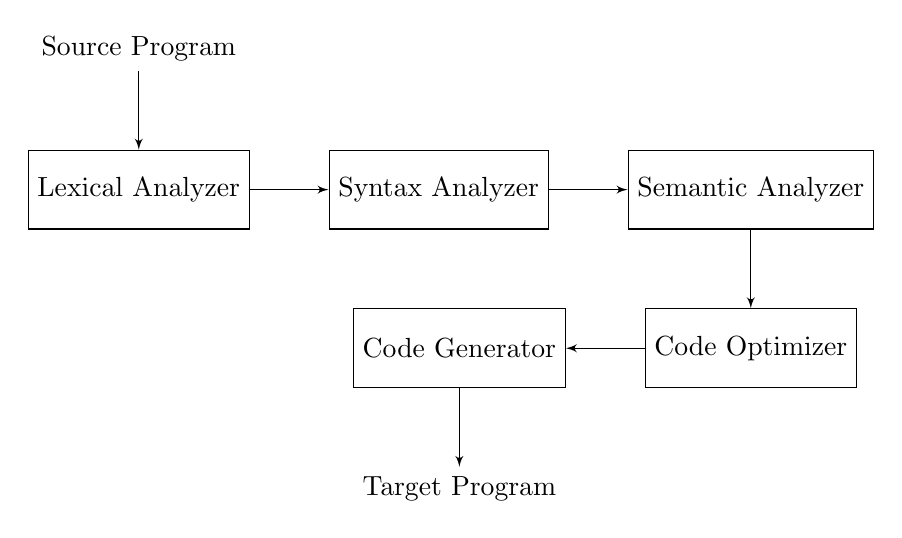
\begin{tikzpicture}[>=latex']
    \tikzset{block/.style= {draw, rectangle, align=center,minimum width=2cm,minimum height=1cm},}

    \node (src) {Source Program};
    \node [block, below =1cm of src] (lex) {Lexical Analyzer};
    \node [block, right =1cm of lex] (syn) {Syntax Analyzer};
    \node [block, right =1cm of syn] (sem) {Semantic Analyzer};
    \node [block, below =1cm of sem] (opt) {Code Optimizer};
    \node [block, left =1cm of opt] (gen) {Code Generator};
    \node [below =1cm of gen] (tar) {Target Program};

    \path[draw,->]
                (src) edge (lex)
                (lex) edge (syn)
                (syn) edge (sem)
                (sem) edge (opt)
                (opt) edge (gen)
                (gen) edge (tar)
                ;
\end{tikzpicture}
\caption{Typical phases of a compiler.}
\label{fig:compiler-architecture}
\end{figure}

However, a compiler is not well suited to use a pipeline architecture.
In general, the modules of a pipeline architecture should be independent of their input source.
This is not the case in compilers, as each phase relies on the completion of the previous phase.
As a result, the input dependencies of a compiler make it too restrictive for a true pipeline architecture.

Instead, compilers are often built as a hybrid of a pipeline architecture and the \textsl{Blackboard Architecture}.
The blackboard architecture consists of;
\begin{itemize}
    \item a knowledge base, the `blackboard',
    \item knowledge sources which use and update the knowledge base, and
    \item a control component to coordinate the operation of knowledge sources.
\end{itemize}

In modern compilers, the data which would be passed through pipes, the Symbol Table and AST,
are used and updated by each phase.
They are subsequently used as the `blackboard'.
Each phase is considered a knowledge source which uses the knowledge base to transform and update the knowledge base.
Finally, in this hybrid, the control component is not required as the sequence of phase execution in a pipeline coordinates operation.
Figure \ref{fig:compiler-architecture-sym} illustrates this proposed architecture.
Of course, there are many compilers out there, many of them deviate from this architectural hybrid.

\begin{figure}[H]
    \centering
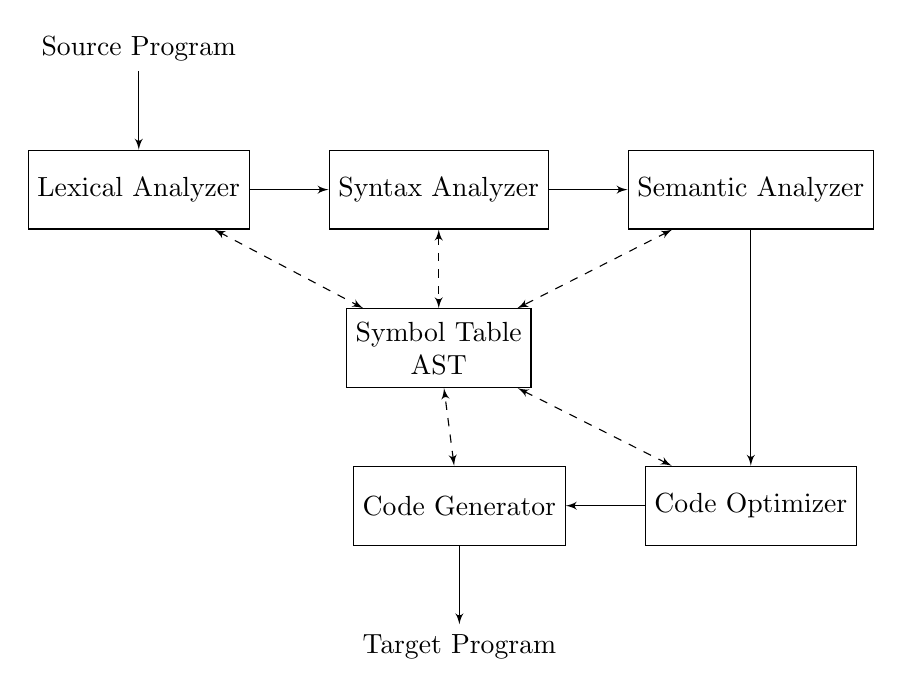
\begin{tikzpicture}[>=latex']
    \tikzset{block/.style= {draw, rectangle, align=center,minimum width=2cm,minimum height=1cm},}

    \node (src) {Source Program};
    \node [block, below =1cm of src] (lex) {Lexical Analyzer};
    \node [block, right =1cm of lex] (syn) {Syntax Analyzer};
    \node [block, right =1cm of syn] (sem) {Semantic Analyzer};
    \node [block, below =3cm of sem] (opt) {Code Optimizer};
    \node [block, left =1cm of opt] (gen) {Code Generator};
    \node [below =1cm of gen] (tar) {Target Program};

    \node [block, below =1cm of syn] (sym) {Symbol Table\\AST};

    \path[draw,->]
                (src) edge (lex)
                (lex) edge (syn)
                (syn) edge (sem)
                (sem) edge (opt)
                (opt) edge (gen)
                (gen) edge (tar)
                ;

    \path[draw,<->,dashed] (lex) edge (sym);
    \path[draw,<->,dashed] (syn) edge (sym);
    \path[draw,<->,dashed] (sem) edge (sym);
    \path[draw,<->,dashed] (opt) edge (sym);
    \path[draw,<->,dashed] (gen) edge (sym);
\end{tikzpicture}
\caption{Phases of a modern compiler.}
\label{fig:compiler-architecture-sym}
\end{figure}

\section{Case Study: MapReduce}

One of the more prevalent uses of the pipeline architecture is the MapReduce pattern.
The MapReduce pattern was discovered in 2004 as a solution to the challenges which Google faced managing their search index \cite{mapreduce}.%
\footnote{Although the pattern was in use prior to their work\cite{mapreduce-critique}} %
MapReduce affords impressive parallelism inherit to the programming pattern.

The two key ideas of MapReduce, are \textsl{map} and \textsl{reduce}.
Below are the generic types of the \textsl{map} and \textsl{reduce} functions in functional programming.

\begin{code}[language=lambda]{}
map : (type$_1$ -> type$_2$) -> type$_1 Seq$ -> type$_2 Seq$
map $f$ $xs$
reduce : (type$_2$ -> type$_1$ -> type$_2$) -> type$_1 Seq$ -> type$_2$ -> type$_2$
reduce $f$ $xs$ $initial$
\end{code}

If you are unfamiliar with this notation, the rough English translation is:
\begin{description}
    \item[map] The parameters of the \textsl{map} function are:
        \begin{enumerate}[label=(\alph*)]
            \item A function, $f$, which takes a parameter of type $\tau_1$ and returns a type $\tau_2$.
            \item A sequence of elements of type $\tau_1$.
        \end{enumerate}
        The return type of the \textsl{map} function is a sequence of elements of type $\tau_2$.
    \item[reduce] The parameters of the \textsl{reduce} function are:
        \begin{enumerate}[label=(\alph*)]
            \item A function, $f$, which takes two parameters, the first of type $\tau_2$ is the current accumulator value, the second of type $\tau_1$ is the current value in the input sequence, and returns a $\tau_2$, the new accumulator value.
            \item A sequence of elements of type $\tau_1$.
            \item An initial accumulator value of type $\tau_2$
        \end{enumerate}
        The return type of the \textsl{reduce} function is the type $\tau_2$.
\end{description}

The code snippet below uses the $map$ and $reduce$ functions
to perform the operations of the above bash example.
One important thing to note about the example below is the map operation on line 11.
Each application of the lambda function within the map operation is completely independent and could,
in theory, be executed simultaneously. 

\begin{code}[language=python,literate={{->}{{$\to$}}{2}{lambda}{{$\lambda$}}{1}},morekeywords={then}]{}
contents = read("assignment.py")

# filter relevant lines by rebuilding the list
contents = reduce(lambda xs x -> 
                      if x.contains("hack")
                        then x + xs
                        else xs,
                    contents,
                    [])

# use map to count occurrences of word
contents = map(lambda line -> line.count("hack"), contents)

# use reduce to sum list of counts
contents = reduce(lambda total curr -> total + curr, contents, 0)

write("code-quality.txt", contents)
\end{code}

So by design, code written in this pattern can process data simultaneously.
Tools such as \link{Hadoop}{https://hadoop.apache.org/} are able to take advantage of this to distribute computation automatically.

\begin{extra}
Using the terminology of a pipeline architecture, what filters do the \textsl{map} and \textsl{reduce} operators roughly correspond to?
\end{extra}

\begin{extra}
How would you improve the efficiency of the code snippet above?
\end{extra}

\bibliographystyle{ieeetr}
\bibliography{articles}

\end{document}